% Table-of-contents graphic for J. Chem. Inf. Model.: exactly 3.25 in x 1.75 in, sans serif, all text >= 6 pt.
% Numbers are from results/paper_values.json (capacity, DOI-grouped, t2): repeated 0.74, new 0.35, share 29%.
% Build: scripts/11_schematics.py (tectonic; writes PDF, PNG and TIF at 600 dpi to paper/figures/).
\documentclass[tikz,border=0pt]{standalone}
\usepackage[T1]{fontenc}
\usepackage{tgheros}
\renewcommand{\familydefault}{\sfdefault}
\usepackage{sansmath}\sansmath
\usetikzlibrary{arrows.meta,calc}

\definecolor{p1}{RGB}{196,82,120}  \definecolor{p1f}{RGB}{250,232,238}
\definecolor{p5}{RGB}{110,84,170}  \definecolor{p5f}{RGB}{238,233,248}
\definecolor{p7}{RGB}{196,96,40}   \definecolor{p7f}{RGB}{251,234,222}
\definecolor{d1}{RGB}{47,93,138} \definecolor{d2}{RGB}{233,128,40} \definecolor{d3}{RGB}{80,160,80}
\definecolor{d4}{RGB}{176,120,160} \definecolor{d6}{RGB}{236,200,60}
\definecolor{d7}{RGB}{150,110,80} \definecolor{d8}{RGB}{185,180,175}
\definecolor{rep}{RGB}{200,60,70} \definecolor{new}{RGB}{90,107,123}

\tikzset{
  six/.style={font=\fontsize{6}{7}\selectfont,align=center},
  sev/.style={font=\fontsize{7}{8.2}\selectfont\bfseries,align=center},
  panel/.style={draw=#1,fill=#1f,line width=0.6pt,rounded corners=3pt},
  sq/.style={minimum size=5.6pt,inner sep=0pt,draw=white,line width=0.3pt},
  arr/.style={-{Stealth[length=4pt,width=4pt]},line width=1.2pt,black!70},
}

\begin{document}
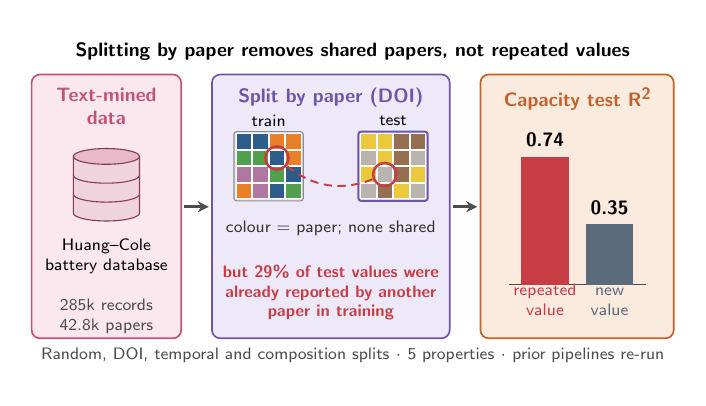
\begin{tikzpicture}[x=1cm,y=1cm]
% exact canvas: 3.25 in x 1.75 in = 8.255 cm x 4.445 cm
\path[use as bounding box] (0,0) rectangle (8.255,4.445);
\fill[white] (0,0) rectangle (8.255,4.445);

% headline
\node[sev,anchor=north] at (4.1275,4.38) {Splitting by paper removes shared papers, not repeated values};

% ---------------- panel 1: database
\draw[panel=p1] (0.05,0.50) rectangle (1.95,3.85);
\node[sev,text=p1,anchor=north] at (1.0,3.80) {Text-mined\\data};
\begin{scope}[shift={(1.0,2.45)}]
  \foreach \yy in {-0.36,-0.12,0.12} {
    \fill[p1!25] (-0.42,\yy) rectangle (0.42,\yy+0.24);
    \fill[p1!25] (0,\yy) ellipse (0.42 and 0.10);
    \draw[p1!70!black,line width=0.4pt] (-0.42,\yy+0.24) -- (-0.42,\yy) arc (180:360:0.42 and 0.10) -- (0.42,\yy+0.24);}
  \fill[p1!40] (0,0.36) ellipse (0.42 and 0.10); \draw[p1!70!black,line width=0.4pt] (0,0.36) ellipse (0.42 and 0.10);
\end{scope}
\node[six,anchor=north] at (1.0,1.88) {Huang--Cole\\battery database};
\node[six,anchor=north,text=black!70] at (1.0,1.12) {285k records\\42.8k papers};

\draw[arr] (1.99,2.17) -- (2.30,2.17);

% ---------------- panel 2: DOI-grouped split
\draw[panel=p5] (2.34,0.50) rectangle (5.36,3.85);
\node[sev,text=p5,anchor=north] at (3.85,3.80) {Split by paper (DOI)};
\newcommand{\grid}[3]{% x, y (top-left square centre), colours
  \begin{scope}[shift={(#1,#2)}]
  \foreach \c [count=\k from 0] in {#3} {
    \pgfmathtruncatemacro{\r}{\k/4}\pgfmathtruncatemacro{\q}{mod(\k,4)}
    \node[sq,fill=\c] at (\q*0.21,-\r*0.21) {};}
  \end{scope}}
\node[six] at (3.06,3.26) {train};  \node[six] at (4.64,3.26) {test};
\grid{2.745}{3.0}{d1,d1,d2,d2,d3,d3,d1,d2,d4,d4,d3,d1,d2,d4,d1,d3}
\grid{4.325}{3.0}{d6,d6,d7,d7,d8,d6,d7,d8,d6,d8,d7,d6,d8,d7,d6,d8}
\draw[black!45,line width=0.4pt,rounded corners=1pt] (2.62,3.125) rectangle (3.50,2.245);
\draw[p5,line width=0.7pt,rounded corners=1pt] (4.20,3.125) rectangle (5.08,2.245);
% the same reported value in a training paper and a test paper
\node[draw=rep,line width=0.9pt,circle,inner sep=0pt,minimum size=8.4pt] (a) at (2.745+0.42,3.0-0.21) {};
\node[draw=rep,line width=0.9pt,circle,inner sep=0pt,minimum size=8.4pt] (b) at (4.325+0.21,3.0-0.42) {};
\draw[rep,line width=0.7pt,densely dashed] (a) to[bend right=30] (b);
\node[six,anchor=north,text=black!80] at (3.85,2.12) {colour = paper; none shared};
\node[six,anchor=north,text=rep,font=\fontsize{6}{7}\selectfont\bfseries] at (3.85,1.55)
  {but 29\% of test values were\\already reported by another\\paper in training};

\draw[arr] (5.40,2.17) -- (5.71,2.17);

% ---------------- panel 3: result
\draw[panel=p7] (5.75,0.50) rectangle (8.205,3.85);
\node[anchor=north,text=p7,font=\fontsize{7}{8.2}\selectfont\bfseries,align=center] at (6.98,3.80) {Capacity test R\raisebox{0.75ex}{\fontsize{6}{6}\selectfont 2}};
\begin{scope}[shift={(6.11,1.18)}]
  \def\H{2.2}
  \draw[black!70,line width=0.4pt] (0,0) -- (1.74,0);
  \fill[rep] (0.16,0) rectangle (0.76,0.74*\H);
  \fill[new] (0.98,0) rectangle (1.58,0.35*\H);
  \node[sev,anchor=south] at (0.46,0.74*\H) {0.74};
  \node[sev,anchor=south] at (1.28,0.35*\H) {0.35};
  \node[six,anchor=north,text=rep,text height=1.5ex] at (0.46,-0.03) {repeated\\value};
  \node[six,anchor=north,text=new,text height=1.5ex] at (1.28,-0.03) {new\\value};
\end{scope}

% footer
\node[six,anchor=south,text=black!70] at (4.1275,0.07)
  {Random, DOI, temporal and composition splits $\cdot$ 5 properties $\cdot$ prior pipelines re-run};
\end{tikzpicture}
\end{document}
